\documentclass[12pt,a4paper]{article}

% --- Packages -----------------------------------------------------------------
\usepackage{fontspec}
\usepackage{polyglossia}
\setdefaultlanguage{russian}
\setotherlanguage{english}

\setmainfont{Times New Roman}
\setmonofont{Menlo}[Scale=0.85]
\newfontfamily\cyrillicfonttt{Menlo}[Scale=0.85]

\usepackage{amsmath,amssymb,amsthm,mathtools}
\usepackage{geometry}
\geometry{a4paper, left=2.5cm, right=2.0cm, top=2.0cm, bottom=2.0cm}
\usepackage{microtype}
\usepackage{xcolor}
\usepackage{tcolorbox}
\tcbuselibrary{breakable,skins}
\usepackage{enumitem}
\setlist{itemsep=2pt,topsep=4pt}
\usepackage{hyperref}
\hypersetup{colorlinks=true,linkcolor=blue!50!black,urlcolor=blue!50!black}
\usepackage{titlesec}
\titleformat{\section}{\normalfont\Large\bfseries}{\thesection}{0.6em}{}
\titleformat{\subsection}{\normalfont\large\bfseries}{\thesubsection}{0.6em}{}
\usepackage{parskip}
\setlength{\parskip}{6pt}
\setlength{\parindent}{0pt}
\usepackage{booktabs}
\usepackage{array}
\usepackage{multirow}
\usepackage{graphicx}
\graphicspath{{figures/}}
\usepackage{float}
\usepackage{caption}
\captionsetup{font=small,labelfont=bf}

% --- Custom commands ----------------------------------------------------------
\newcommand{\R}{\mathbb{R}}
\newcommand{\E}{\mathbb{E}}
\newcommand{\sign}{\operatorname{sign}}
\newcommand{\argmax}{\operatorname{arg\,max}}
\newcommand{\argmin}{\operatorname{arg\,min}}
\DeclareMathOperator{\Loss}{Loss}
\DeclareMathOperator{\hinge}{hinge}

% Intuition box
\newtcolorbox{intuition}[1][]{
  enhanced,breakable,
  colback=blue!4,colframe=blue!50!black,
  boxrule=0.5pt,arc=2pt,
  title=Интуиция,
  fonttitle=\bfseries,
  #1
}
\newtcolorbox{derivation}[1][]{
  enhanced,breakable,
  colback=gray!5,colframe=gray!50!black,
  boxrule=0.5pt,arc=2pt,
  title=Вывод,
  fonttitle=\bfseries,
  #1
}
\newtcolorbox{example}[1][]{
  enhanced,breakable,
  colback=green!3,colframe=green!40!black,
  boxrule=0.5pt,arc=2pt,
  title=Численный пример,
  fonttitle=\bfseries,
  #1
}
\newtcolorbox{warning}[1][]{
  enhanced,breakable,
  colback=red!3,colframe=red!50!black,
  boxrule=0.5pt,arc=2pt,
  title=Тонкий момент,
  fonttitle=\bfseries,
  #1
}

\title{\textbf{Приложение к ЛР-4}\\\large Машины опорных векторов и алгоритм Pegasos:\\интуиция, выводы и численные примеры}
\author{Пахомов В.В., группа P3324}
\date{}

\begin{document}
\maketitle

\begin{abstract}
\noindent Это приложение к лабораторной работе разбирает математику SVM и алгоритма Pegasos с нуля. Мы пройдём от геометрической идеи разделяющей гиперплоскости до конкретной формулы обновления весов в коде, проследим, откуда берётся каждый множитель, и посчитаем 2 итерации Pegasos руками на маленьком примере. Цель документа~--- сделать так, чтобы формулы из основного отчёта перестали быть страшными и стали логичным следствием простой геометрической идеи.
\end{abstract}

\tableofcontents
\vspace{0.5cm}

% ==============================================================================
\section{Зачем нужен SVM и какую задачу он решает}

У нас есть набор объектов $x_1, \ldots, x_n \in \R^d$ (в нашем случае $d = 90$~--- средние амплитуды по 18 каналам и 5 временным окнам) и метки $y_i \in \{-1, +1\}$ (Target / NonTarget). Нужно найти функцию $f\colon \R^d \to \{-1, +1\}$, которая по новому объекту скажет его класс.

\textbf{Линейный классификатор} это самый простой выбор:
\[
  f(x) = \sign(w \cdot x + b),
\]
где $w \in \R^d$~--- вектор весов, $b \in \R$~--- смещение, $w \cdot x = \sum_j w_j x_j$~--- обычное скалярное произведение.

Геометрически уравнение $w \cdot x + b = 0$ задаёт \emph{гиперплоскость} (в 2D это прямая, в 3D~--- плоскость, в $d$-мерном~--- $(d{-}1)$-мерная плоскость). Точки, у которых $w \cdot x + b > 0$, лежат по одну сторону~--- мы говорим $f(x) = +1$. У которых $< 0$~--- по другую, $f(x) = -1$.

\begin{intuition}
Представьте 2D-плоскость с двумя облаками точек: красные слева, синие справа. Между ними можно провести бесконечно много прямых, разделяющих классы. SVM ищет ту, которая лежит \textbf{ровно посередине} и максимально далеко от обоих облаков. Это даёт ей лучшую способность обобщать: малое возмущение объекта не пересечёт границу.
\end{intuition}

\begin{figure}[H]
  \centering
  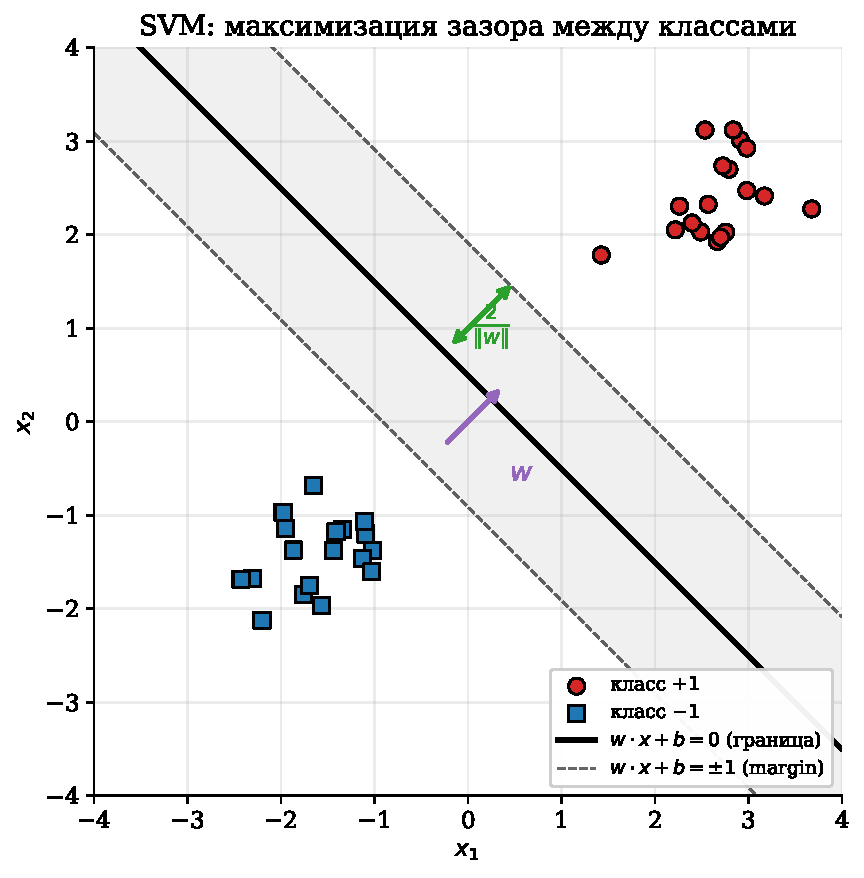
\includegraphics[width=0.78\linewidth]{svm_geometry.pdf}
  \caption{Геометрический смысл SVM: чёрная линия~--- разделяющая гиперплоскость $w \cdot x + b = 0$, пунктирные~--- параллельные ей плоскости $w \cdot x + b = \pm 1$. Зазор между ними равен $2/\|w\|$, и SVM максимизирует это расстояние. Вектор $w$ перпендикулярен границе.}
\end{figure}

% ==============================================================================
\section{Геометрический смысл: максимизация зазора (margin)}

\subsection{Что такое зазор}

Возьмём гиперплоскость $H = \{x \in \R^d : w \cdot x + b = 0\}$. Расстояние от произвольной точки $x_i$ до этой гиперплоскости считается по формуле:
\[
  d(x_i, H) = \frac{|w \cdot x_i + b|}{\|w\|},
\]
где $\|w\| = \sqrt{w_1^2 + \cdots + w_d^2}$~--- евклидова норма.

\begin{derivation}
Откуда берётся $\|w\|$ в знаменателе. Вектор $w$ перпендикулярен гиперплоскости (это базовое свойство уравнения $w \cdot x + b = 0$). Если из точки $x_i$ опустить перпендикуляр на $H$, то он пойдёт вдоль $w/\|w\|$~--- единичного направления. Длина проекции вектора $x_i - x_0$ (где $x_0$~--- любая точка на $H$) на это направление:
\[
  \frac{(x_i - x_0) \cdot w}{\|w\|} = \frac{w \cdot x_i - w \cdot x_0}{\|w\|} = \frac{w \cdot x_i + b}{\|w\|},
\]
так как $w \cdot x_0 = -b$ для любой точки на гиперплоскости. Модуль берётся, чтобы расстояние было неотрицательным.
\end{derivation}

\textbf{Зазор} (margin) объекта $x_i$ с меткой $y_i \in \{-1, +1\}$ это знаковое расстояние:
\[
  \gamma_i = \frac{y_i (w \cdot x_i + b)}{\|w\|}.
\]

Если $\gamma_i > 0$, точка классифицирована верно (метка совпадает со стороной). Если $\gamma_i < 0$~--- ошибка. Величина $|\gamma_i|$~--- это насколько \emph{уверенно} классификатор отвечает: чем больше, тем дальше точка от границы.

\subsection{Задача максимизации зазора}

SVM хочет максимизировать минимальный по выборке зазор:
\[
  \max_{w, b} \min_{i=1,\ldots,n} \frac{y_i (w \cdot x_i + b)}{\|w\|}.
\]

Эта формулировка имеет неприятную особенность: если умножить $w$ и $b$ на любое положительное число $c > 0$, гиперплоскость не изменится, но числитель и знаменатель умножатся на $c$, и значение зазора останется тем же. То есть оптимум не единственен.

\textbf{Стандартный фикс}~--- зафиксировать масштаб условием $\min_i y_i(w \cdot x_i + b) = 1$. Это значит, что ближайшие к границе точки имеют ненормированный зазор ровно $1$, а минимальный нормированный зазор тогда $1/\|w\|$. Максимизировать $1/\|w\|$~--- то же, что минимизировать $\|w\|^2 / 2$.

Получаем классическую формулировку SVM (hard-margin):
\[
  \min_{w, b} \tfrac{1}{2}\|w\|^2
  \quad \text{при условиях} \quad
  y_i (w \cdot x_i + b) \ge 1 \;\; \forall i.
\]

\begin{intuition}
$\|w\|^2$ маленькое $\Leftrightarrow$ $1/\|w\|$ большое $\Leftrightarrow$ зазор большой. Поэтому минимизация $\|w\|^2$~--- это \textbf{и есть} максимизация зазора при фиксированном условии $y_i(w \cdot x_i + b) \ge 1$.

Иногда новички думают, что $\|w\|^2$~--- какая-то непонятная «регуляризация для борьбы с переобучением». На самом деле для SVM это не дополнительная штука, а ядро самой геометрической постановки.
\end{intuition}

% ==============================================================================
\section{Soft-margin и hinge loss}

\subsection{Что делать, если данные не разделимы}

Hard-margin SVM требует, чтобы \emph{все} объекты лежали правильно с зазором $\ge 1$. На реальных данных (особенно EEG, где шум большой) это невозможно. Идея soft-margin: разрешить нарушения, но штрафовать за них.

Введём \textbf{слабые переменные} $\xi_i \ge 0$, которые показывают, насколько объект $i$ нарушает условие зазора:
\[
  y_i (w \cdot x_i + b) \ge 1 - \xi_i.
\]

Если $\xi_i = 0$, объект классифицирован верно с правильным зазором. Если $0 < \xi_i < 1$~--- классифицирован верно, но внутри margin-полосы. Если $\xi_i \ge 1$~--- классифицирован неверно. Целевая функция теперь штрафует $\xi_i$:
\[
  \min_{w, b, \xi} \tfrac{1}{2}\|w\|^2 + C \sum_{i=1}^n \xi_i,
  \quad \xi_i \ge 0, \;\; y_i(w \cdot x_i + b) \ge 1 - \xi_i.
\]

$C > 0$~--- параметр, балансирующий: \textbf{большое $C$} = жёстко штрафуем ошибки, узкий margin, риск переобучения; \textbf{малое $C$} = мягко, широкий margin, может недообучить.

\subsection{От slack-переменных к hinge loss}

Минимальное $\xi_i \ge 0$, удовлетворяющее $\xi_i \ge 1 - y_i(w \cdot x_i + b)$, это:
\[
  \xi_i^* = \max\bigl(0,\; 1 - y_i(w \cdot x_i + b)\bigr).
\]

Подставив в целевую функцию, получаем \textbf{безусловную задачу}:
\[
  \boxed{\;
    \min_{w,b} \;
    \tfrac{1}{2}\|w\|^2 + C \sum_{i=1}^n \max\bigl(0,\; 1 - y_i(w \cdot x_i + b)\bigr)
  \;}
\]

Функция $\max(0,\, 1 - m)$, где $m = y_i(w \cdot x_i + b)$~--- это и есть \textbf{hinge loss} (loss «петлёй»):
\[
  \ell_{\hinge}(m) = \max(0,\, 1 - m) =
  \begin{cases}
    0, & m \ge 1 \quad (\text{зазор $\ge 1$, штраф нулевой})\\
    1 - m, & m < 1 \quad (\text{штраф растёт линейно})
  \end{cases}
\]

\begin{intuition}
График hinge loss:
\begin{itemize}
  \item На $m \ge 1$ ровный нуль: объект далеко за границей с правильной стороны, всё хорошо.
  \item На $0 \le m < 1$: правильно классифицирован, но внутри margin-полосы. Штраф растёт.
  \item На $m < 0$: ошибка, штраф $> 1$, растёт линейно.
\end{itemize}
В точке $m = 1$ есть «излом», производная не существует. Это важно для алгоритма~--- понадобится \emph{субградиент} вместо обычного градиента.
\end{intuition}

\begin{figure}[H]
  \centering
  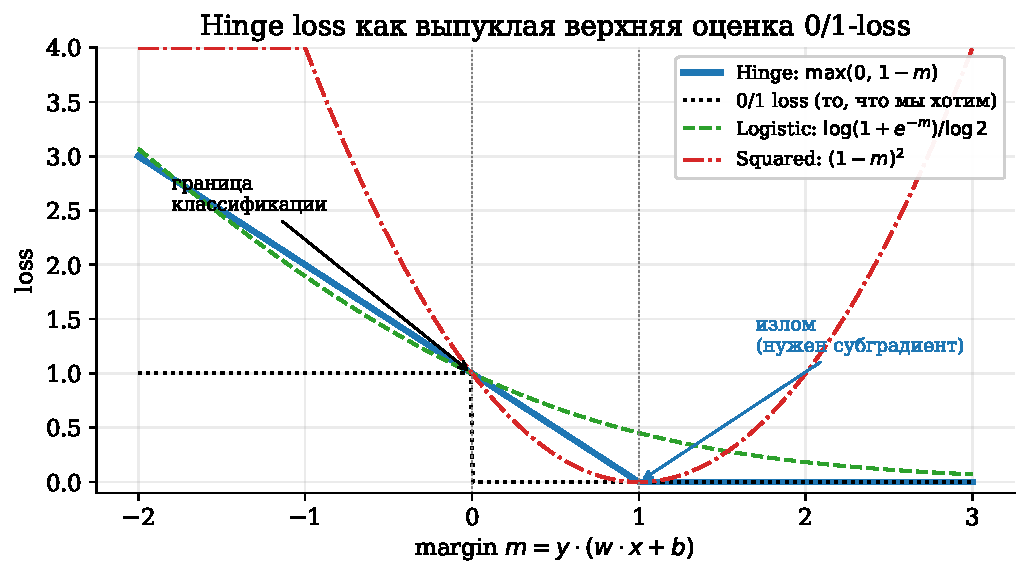
\includegraphics[width=0.85\linewidth]{hinge_loss.pdf}
  \caption{Hinge loss как функция margin'а $m = y(w \cdot x + b)$. Чёрный пунктир~--- «правильный» 0/1 loss, который мы хотим минимизировать, но не можем (он недифференцируем и не выпуклый). Hinge~--- его выпуклая верхняя оценка. На $m \ge 1$ штраф ноль (объект далеко за margin), при $m < 1$ растёт линейно. В точке $m = 1$ излом~--- именно поэтому в Pegasos используется субградиент. Для сравнения показаны logistic loss (что использует логрег) и квадратичный loss.}
\end{figure}

В отчёте используется нормировка на $n$ и параметр $\lambda = 1/C$ вместо $C$. Это эквивалентно с точностью до масштаба:
\[
  L(w, b) = \tfrac{\lambda}{2}\|w\|^2 + \tfrac{1}{n}\sum_{i=1}^n \max\bigl(0,\, 1 - y_i(w \cdot x_i + b)\bigr).
\]

При $C = 1$ имеем $\lambda = 1$, то есть оба слагаемых в нашей реализации идут с равным весом.

% ==============================================================================
\section{Pegasos: стохастический субградиентный спуск}

\subsection{Что такое субградиент}

Hinge $\ell(m) = \max(0,\, 1 - m)$ не дифференцируем в точке $m = 1$. Слева производная $-1$, справа $0$. \textbf{Субградиент}~--- это любое значение между ними (включая концы):
\[
  \partial \ell(m) =
  \begin{cases}
    \{-1\}, & m < 1\\
    [-1, 0], & m = 1\\
    \{0\}, & m > 1
  \end{cases}
\]

В алгоритме мы выбираем удобный элемент субградиента. На границе $m = 1$ берём $0$~--- это даёт более «гладкое» поведение. То есть на практике:
\[
  \frac{\partial \ell_i}{\partial w} =
  \begin{cases}
    -y_i x_i, & y_i(w \cdot x_i + b) < 1 \quad \text{(объект внутри margin)}\\
    0, & \text{иначе}
  \end{cases}
\]
\[
  \frac{\partial \ell_i}{\partial b} =
  \begin{cases}
    -y_i, & y_i(w \cdot x_i + b) < 1\\
    0, & \text{иначе}
  \end{cases}
\]

\begin{derivation}
Вычислим градиент $\ell_i = \max(0,\, 1 - y_i(w \cdot x_i + b))$ по $w$ на участке $m < 1$ (то есть $1 - m > 0$, hinge активен):
\[
  \frac{\partial}{\partial w}\bigl(1 - y_i(w \cdot x_i + b)\bigr)
  = -y_i\, \frac{\partial(w \cdot x_i)}{\partial w}
  = -y_i\, x_i.
\]
По $b$ аналогично: $\partial/\partial b\, (1 - y_i(w \cdot x_i + b)) = -y_i$.

Регуляризация $\tfrac{\lambda}{2}\|w\|^2$ даёт $\partial/\partial w = \lambda w$ (по $b$ зависимости нет).
\end{derivation}

\subsection{Полный градиент по объёму $n$}

Если бы мы хотели делать честный градиентный спуск, надо было бы суммировать по всем $n$ объектам:
\[
  \nabla_w L = \lambda w - \frac{1}{n}\sum_{i: m_i < 1} y_i x_i.
\]

Для $n = 1728$ это нормально, но для миллиона объектов уже тяжело. Pegasos предлагает \textbf{стохастическую} версию: на каждой итерации берём \emph{один случайный} объект, считаем градиент по нему и шагаем.

\subsection{Алгоритм Pegasos шаг за шагом}

\textbf{Инициализация:} $w_1 = 0$, $b_1 = 0$.

\textbf{На итерации $t = 1, 2, \ldots, T$:}
\begin{enumerate}
  \item Выбрать случайный индекс $i \in \{1, \ldots, n\}$.
  \item Вычислить шаг обучения $\eta_t = \dfrac{1}{\lambda\, t}$ (убывает по гиперболе).
  \item Вычислить margin $m_i = y_i(w_t \cdot x_i + b_t)$.
  \item \textbf{Если} $m_i < 1$ (hinge активен):
    \[
      w_{t+1} = (1 - \eta_t \lambda) w_t + \eta_t\, y_i\, x_i,
      \qquad b_{t+1} = b_t + \eta_t\, y_i.
    \]
  \item \textbf{Иначе} (объект далеко за margin, hinge $= 0$):
    \[
      w_{t+1} = (1 - \eta_t \lambda) w_t, \qquad b_{t+1} = b_t.
    \]
\end{enumerate}

\subsection{Откуда взялся множитель $(1 - \eta_t \lambda)$}

Стандартный шаг градиентного спуска для одной точки:
\[
  w_{t+1} = w_t - \eta_t \nabla_w \ell_i(w_t).
\]

Здесь $\nabla_w \ell_i$~--- градиент \emph{полного} loss по одному объекту, включая регуляризацию:
\[
  \nabla_w \ell_i = \lambda w_t + \begin{cases} -y_i x_i, & m_i < 1\\ 0, & m_i \ge 1\end{cases}
\]

Подставляем:
\[
  w_{t+1} = w_t - \eta_t \bigl(\lambda w_t \;-\; y_i x_i \cdot [m_i < 1]\bigr)
  = (1 - \eta_t \lambda) w_t + \eta_t y_i x_i \cdot [m_i < 1].
\]

Множитель $(1 - \eta_t \lambda)$~--- это \textbf{сжатие весов}, происходящее каждую итерацию от регуляризации $\lambda$. Это работает как «забывание»: каждый шаг текущий $w$ слегка сжимается к нулю, тем самым $\|w\|$ остаётся ограниченной. Прибавление $\eta_t y_i x_i$ происходит только когда объект внутри margin~--- это «коррекция в сторону этого объекта».

\subsection{Почему $\eta_t = 1/(\lambda t)$}

Это не магия~--- это \textbf{оптимальная} скорость для сильно выпуклых функций. Целевая функция:
\[
  L(w) = \tfrac{\lambda}{2}\|w\|^2 + \tfrac{1}{n}\sum \ell_i(w)
\]
сильно выпукла с параметром $\lambda$ (из-за квадратичного члена $\lambda/2 \cdot \|w\|^2$). Теория стохастического градиентного спуска говорит, что для $\lambda$-сильно выпуклых функций оптимальный шаг $\eta_t = c/(\lambda t)$ даёт скорость сходимости $\E[L(w_T)] - L(w^*) = O(\log T / T)$.

\begin{intuition}
Шаг должен убывать, иначе $w$ будет «прыгать» вокруг оптимума и не сойдётся. Но не слишком быстро~--- иначе остановимся, не дойдя до оптимума.

$1/t$~--- золотая середина: суммарный путь $\sum_t 1/t$ расходится (медленно, как $\log T$), значит мы можем добраться куда угодно, но скорость убывает, поэтому колебания вокруг оптимума затухают.
\end{intuition}

\begin{figure}[H]
  \centering
  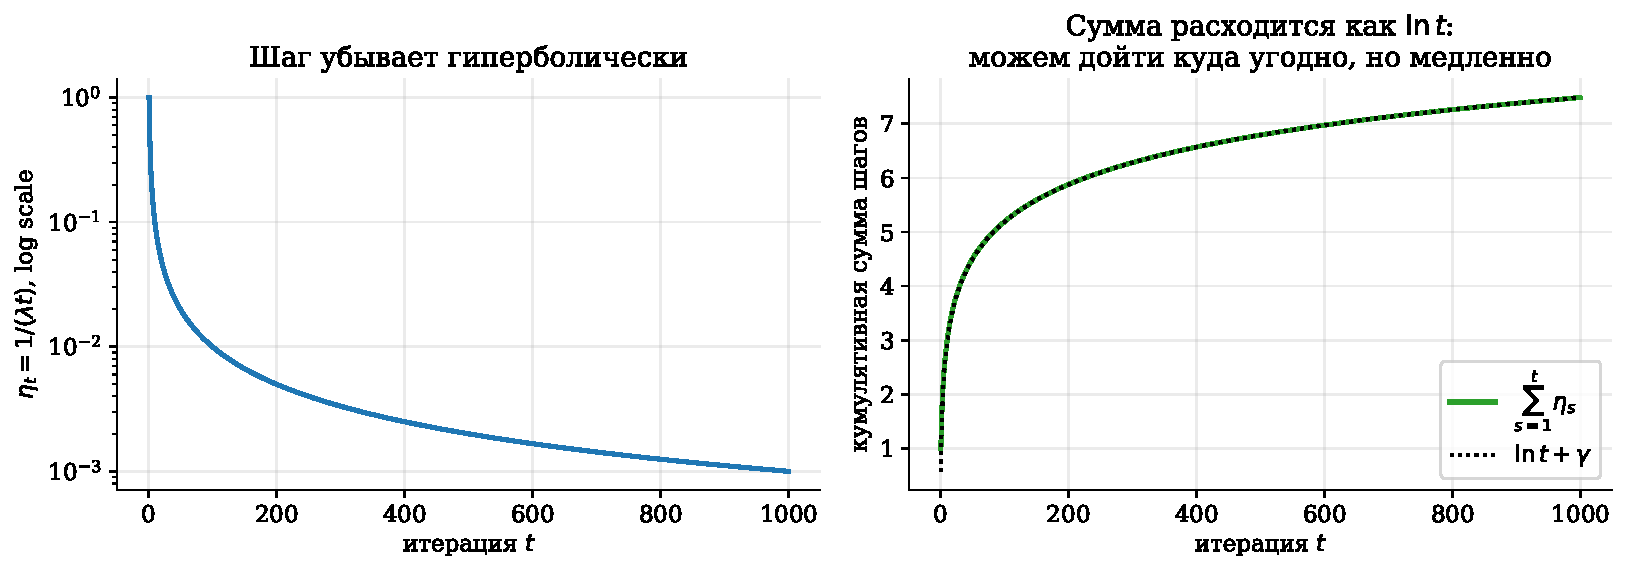
\includegraphics[width=0.95\linewidth]{eta_schedule.pdf}
  \caption{Слева: $\eta_t = 1/(\lambda t)$ убывает гиперболически (log-шкала по~$y$). Справа: кумулятивная сумма $\sum_{s=1}^t \eta_s$ растёт как $\ln t$~--- расходящийся, но очень медленно. Это идеальный баланс: бесконечное число шагов даёт неограниченный пробег, но колебания вокруг оптимума затухают.}
\end{figure}

% ==============================================================================
\section{Численный пример: 2 итерации Pegasos руками}

Возьмём игрушечную задачу в 2D. Четыре точки, два класса:
\begin{center}
\begin{tabular}{cccc}
\toprule
$i$ & $x_i$ & $y_i$ & описание\\
\midrule
1 & $(2, 1)$ & $+1$ & Target справа сверху\\
2 & $(3, 2)$ & $+1$ & Target справа сверху\\
3 & $(-1, -1)$ & $-1$ & NonTarget слева снизу\\
4 & $(-2, 0)$ & $-1$ & NonTarget слева снизу\\
\bottomrule
\end{tabular}
\end{center}

Параметры: $\lambda = 1$, $w_1 = (0, 0)$, $b_1 = 0$.

\textbf{Итерация $t = 1$.} $\eta_1 = 1/(\lambda \cdot 1) = 1$.

Случайно выбрали $i = 1$, объект $x_1 = (2, 1)$, $y_1 = +1$.

Margin: $m_1 = y_1(w_1 \cdot x_1 + b_1) = 1 \cdot (0 \cdot 2 + 0 \cdot 1 + 0) = 0$. Это $< 1$, hinge активен.

Обновление:
\[
  w_2 = (1 - 1 \cdot 1) \cdot (0, 0) + 1 \cdot 1 \cdot (2, 1) = (0, 0) + (2, 1) = (2, 1).
\]
\[
  b_2 = 0 + 1 \cdot 1 = 1.
\]

\textbf{Итерация $t = 2$.} $\eta_2 = 1/(1 \cdot 2) = 0{,}5$.

Случайно выбрали $i = 3$, объект $x_3 = (-1, -1)$, $y_3 = -1$.

Margin: $m_3 = -1 \cdot (2 \cdot (-1) + 1 \cdot (-1) + 1) = -1 \cdot (-2 - 1 + 1) = -1 \cdot (-2) = 2$. Это $> 1$~--- объект уже хорошо классифицирован, hinge неактивен.

Обновление (только сжатие):
\[
  w_3 = (1 - 0{,}5 \cdot 1) \cdot (2, 1) = 0{,}5 \cdot (2, 1) = (1, 0{,}5).
\]
\[
  b_3 = 1.
\]

\begin{example}
После двух итераций граница: $1 \cdot x_1 + 0{,}5 \cdot x_2 + 1 = 0$, или $x_2 = -2 x_1 - 2$. Эта прямая отделяет $\{x_1, x_2\}$ от $\{x_3, x_4\}$ верно, и зазор уже есть. Каждая следующая итерация будет уточнять её.

\textbf{Этот процесс на практике} выглядит как на рисунке ниже: уже после 100 итераций граница становится хорошо центрированной, а к 1500 итерациям margin прижимается к ближайшим точкам каждого класса:

\begin{figure}[H]
  \centering
  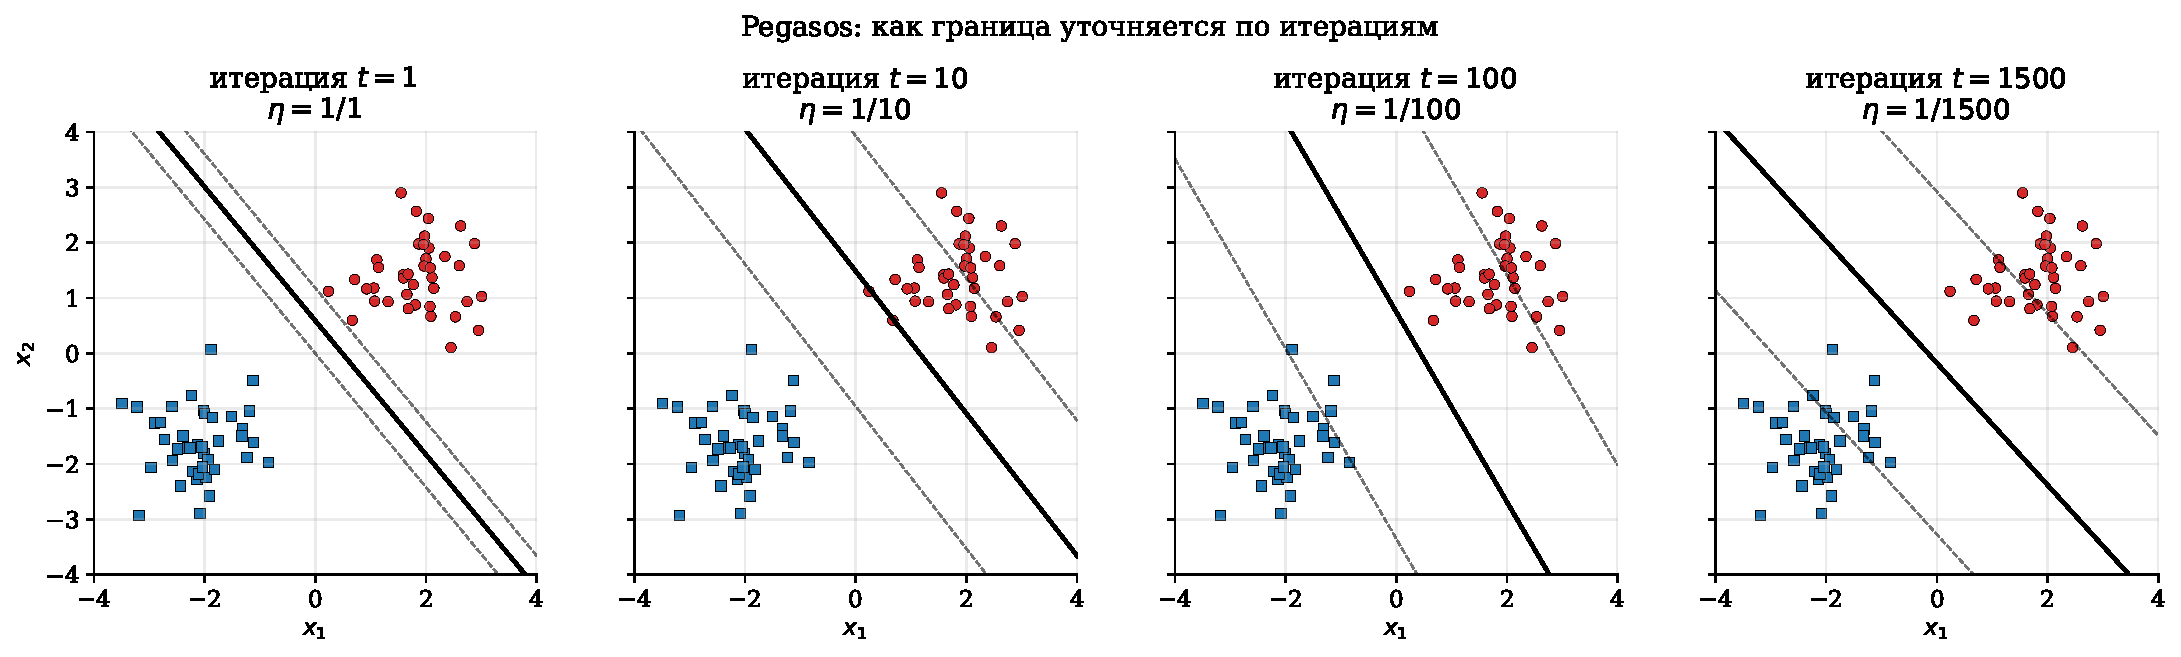
\includegraphics[width=1.0\linewidth]{pegasos_evolution.pdf}
  \caption{Pegasos на двух классах. Сплошная линия~--- граница $w \cdot x + b = 0$, пунктир~--- параллельные $\pm 1$-плоскости (margin). На итерации 1 граница случайна (мы видели один объект), на 10 уже грубо в правильную сторону, на 100 близка к финальной, на 1500 margin прижимается к ближайшим точкам.}
\end{figure}

Заметьте: на шаге~2 \textbf{веса уменьшились} (с $(2,1)$ до $(1; 0{,}5)$), хотя мы ничего не «выучили нового». Это работает регуляризация. Если бы мы не встречали больше объектов внутри margin, $w$ постепенно сжимался бы к нулю~--- именно это и есть смысл регуляризации.
\end{example}

% ==============================================================================
\section{Связь $\{0,1\} \to \{-1,+1\}$}

В коде есть строка:
\begin{quote}
\texttt{y\_train\_svm = 2 * y\_train - 1}
\end{quote}

Это переводит метки. Откуда: если $y \in \{0, 1\}$, то $2y - 1 \in \{-1, +1\}$. Зачем это нужно?

Hinge loss $\max(0, 1 - y \cdot (w \cdot x + b))$ имеет смысл только для $y \in \{-1, +1\}$. Если бы мы оставили $y \in \{0, 1\}$, то для отрицательного класса $y = 0$ выражение $y \cdot (w \cdot x + b) = 0$, и hinge $= \max(0, 1 - 0) = 1$ \emph{всегда} (независимо от предсказания), что бессмысленно.

При $y \in \{-1, +1\}$ всё работает: для положительного класса хотим $w \cdot x + b > 0$ (margin $> 0$), для отрицательного $w \cdot x + b < 0$, и $y \cdot (w \cdot x + b) > 0$ в обоих случаях, когда ответ верный.

% ==============================================================================
\section{Метрики качества и ROC-кривая}

\subsection{Матрица ошибок и базовые метрики}

После предсказания $\hat{y}$ на тесте формируется матрица $2 \times 2$:

\begin{center}
\begin{tabular}{cc|cc}
& & \multicolumn{2}{c}{Предсказано}\\
& & + & −\\\hline
\multirow{2}{*}{Истина} & + & TP & FN\\
& − & FP & TN\\
\end{tabular}
\end{center}

\begin{itemize}
  \item \textbf{TP} (true positive)~--- истинно положительный: $y = 1$, $\hat{y} = 1$.
  \item \textbf{TN} (true negative)~--- истинно отрицательный.
  \item \textbf{FP} (false positive, ошибка I рода)~--- $y = 0$, $\hat{y} = 1$.
  \item \textbf{FN} (false negative, ошибка II рода)~--- $y = 1$, $\hat{y} = 0$.
\end{itemize}

Метрики:
\begin{align*}
  \text{Accuracy} &= \frac{TP + TN}{TP + TN + FP + FN} \quad \text{(доля верных, обманчива при дисбалансе)}\\
  \text{Precision} &= \frac{TP}{TP + FP} \quad \text{(точность: доля верных среди предсказанных +)}\\
  \text{Recall} &= \frac{TP}{TP + FN} \quad \text{(полнота: доля найденных среди истинных +)}\\
  F_1 &= \frac{2 \cdot \text{Precision} \cdot \text{Recall}}{\text{Precision} + \text{Recall}} \quad \text{(гармоническое среднее)}
\end{align*}

\begin{intuition}
Зачем precision и recall, если есть accuracy? В нашей задаче P300 истинных Target всего 1 из 6 эпох. Тривиальный классификатор «всегда NonTarget» даёт accuracy $\approx 0{,}83$~--- звучит хорошо, но мы вообще не нашли ни одного Target! Поэтому:
\begin{itemize}
  \item \textbf{Recall} говорит, сколько Target мы поймали из всех настоящих. Низкий recall = пропустили P300-вспышки.
  \item \textbf{Precision} говорит, насколько мы доверяем нашему «Target»-предсказанию. Низкий precision = много ложных тревог.
  \item \textbf{F1} штрафует за провал в любой из двух~--- хорошее единое число для дисбалансных задач.
\end{itemize}
\end{intuition}

\subsection{Macro vs micro усреднение}

Для бинарной задачи macro считает precision/recall для каждого класса отдельно и усредняет с равным весом. Это правильно при дисбалансе: важно качество \emph{обоих} классов одинаково.

\subsection{ROC-кривая и AUC}

SVM возвращает не только метку, но и \emph{уверенность}~--- значение $w \cdot x + b$ (decision function). Чем больше, тем сильнее модель уверена в положительном классе. Можем варьировать порог $\tau$ и считать предсказанием $\hat{y} = +1 \iff w \cdot x + b > \tau$.

При разных $\tau$ получаются разные TPR и FPR:
\[
  \text{TPR} = \frac{TP}{TP + FN} = \text{Recall}, \qquad \text{FPR} = \frac{FP}{FP + TN}.
\]

\begin{itemize}
  \item При $\tau = -\infty$ всё предсказано $+$: $TP = $ все Target, $FP = $ все NonTarget. TPR $= 1$, FPR $= 1$.
  \item При $\tau = +\infty$ всё $-$: $TP = 0$, $FP = 0$. TPR $= 0$, FPR $= 0$.
\end{itemize}

\textbf{ROC-кривая}~--- параметрическая кривая $\bigl(\text{FPR}(\tau), \text{TPR}(\tau)\bigr)$ при пробегании $\tau$ от $+\infty$ до $-\infty$. Она идёт из $(0,0)$ в $(1,1)$.

\textbf{AUC} (Area Under Curve)~--- площадь под этой кривой:
\begin{itemize}
  \item $\text{AUC} = 1$~--- идеальный классификатор (есть такой порог, при котором TPR $=1$, FPR $=0$).
  \item $\text{AUC} = 0{,}5$~--- случайный (кривая = диагональ $y = x$).
  \item $\text{AUC} < 0{,}5$~--- хуже случайного (можно инвертировать метки).
\end{itemize}

\textbf{Вероятностная интерпретация AUC.} Возьмём случайный объект $x^+$ из класса $+$ и случайный $x^-$ из класса $-$. AUC~--- это вероятность, что классификатор поставит $x^+$ выше:
\[
  \text{AUC} = \Pr\bigl(f(x^+) > f(x^-)\bigr).
\]

То есть AUC = 0,995 в нашей задаче значит: в 99,5\% случаев случайный Target ранжируется выше случайного NonTarget.

\begin{figure}[H]
  \centering
  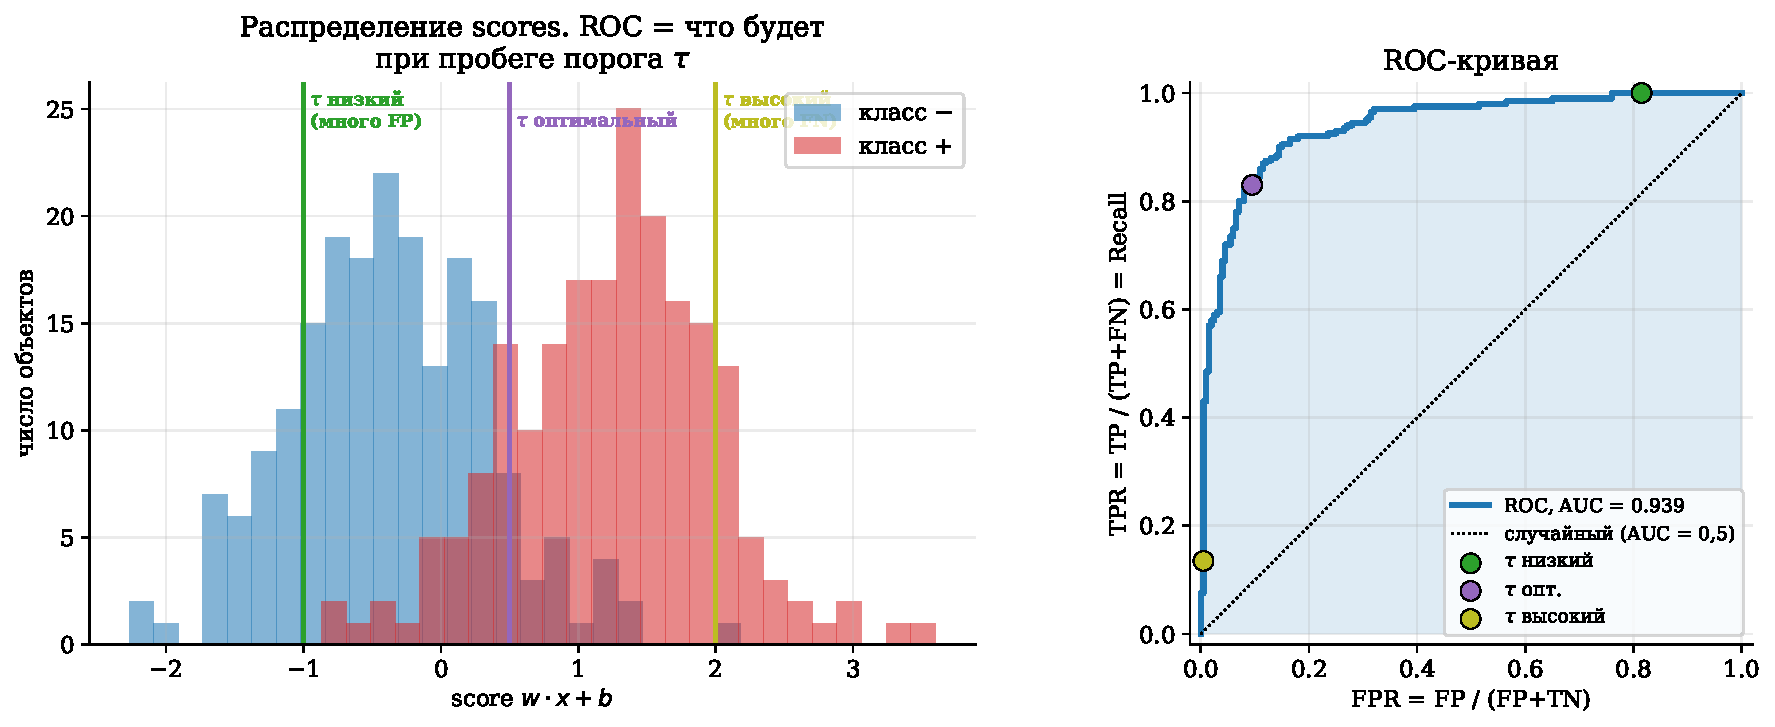
\includegraphics[width=1.0\linewidth]{roc_intuition.pdf}
  \caption{Что такое ROC-кривая. Слева: распределения scores $w \cdot x + b$ для двух классов. Три порога $\tau$ показывают разные trade-off: низкий ловит почти всех Target ценой ложных тревог, высокий~--- мало ложных, но много пропусков. Справа: соответствующая ROC. Каждая точка кривой~--- результат одного порога; AUC~--- площадь под всей кривой и не зависит от выбора $\tau$.}
\end{figure}

\subsection{Sigmoid для перевода в вероятности}

В коде используется
\[
  \hat{p}(x) = \frac{1}{1 + e^{-(w \cdot x + b)}}.
\]

Это \emph{искусственная} калибровка~--- SVM не возвращает вероятности по построению, в отличие от логистической регрессии. Для ROC-кривой подходит \emph{любая} монотонная функция от $w \cdot x + b$, так что сигмоида не меняет ROC (поэтому AUC одинаков с просто decision function).

% ==============================================================================
\section{Что важно запомнить}

\begin{itemize}
  \item SVM ищет гиперплоскость, максимизирующую \textbf{зазор} (margin), то есть расстояние от границы до ближайших точек.
  \item Минимизация $\|w\|^2$~--- это \emph{не дополнительная} регуляризация, а сама математическая постановка максимизации margin'а.
  \item Soft-margin вводит slack-переменные, и они превращаются в \textbf{hinge loss} $\max(0, 1 - m)$.
  \item Hinge не дифференцируем в одной точке, поэтому Pegasos использует \textbf{субградиент}.
  \item Формула Pegasos $w \leftarrow (1 - \eta\lambda)w + \eta y x$~--- это просто стохастический градиент с регуляризацией.
  \item $\eta_t = 1/(\lambda t)$~--- оптимальная скорость для сильно выпуклых задач.
  \item Метки $\{0,1\} \to \{-1,+1\}$~--- из-за устройства hinge loss.
  \item AUC~--- вероятность правильного ранжирования случайной пары $(x^+, x^-)$, не зависит от выбора порога.
\end{itemize}

\end{document}
